%第2章:準備
本章では本研究で使用した用語、技術について述べる。本研究はV字モデルに従って開発を行い、設計に関してはUML言語を用いた。実装部分の画像処理ではYoloとpyzbarを使用した。以下にそれぞれの用語の開発と、本研究との関連も込めて述べる。V字モデルと設計に関する用語は2.1節で述べ、画像処理に関わる用語と技術の説明は2.2節に述べた。

\section{設計に用いた用語解説}

\subsection*{V字モデル}
V字モデルとはシステム開発を要求分析、基本設計、詳細設計、実装に分けて時間軸順に検証、テストを行う開発プロセスである。細かく要素ごとにテストをしていくことで、開発の途中で大幅な変更や問題が起きにくくなる利点がある。本研究ではV字モデルに従って、開発を行っている。

\begin{figure}[htbp]
\centering
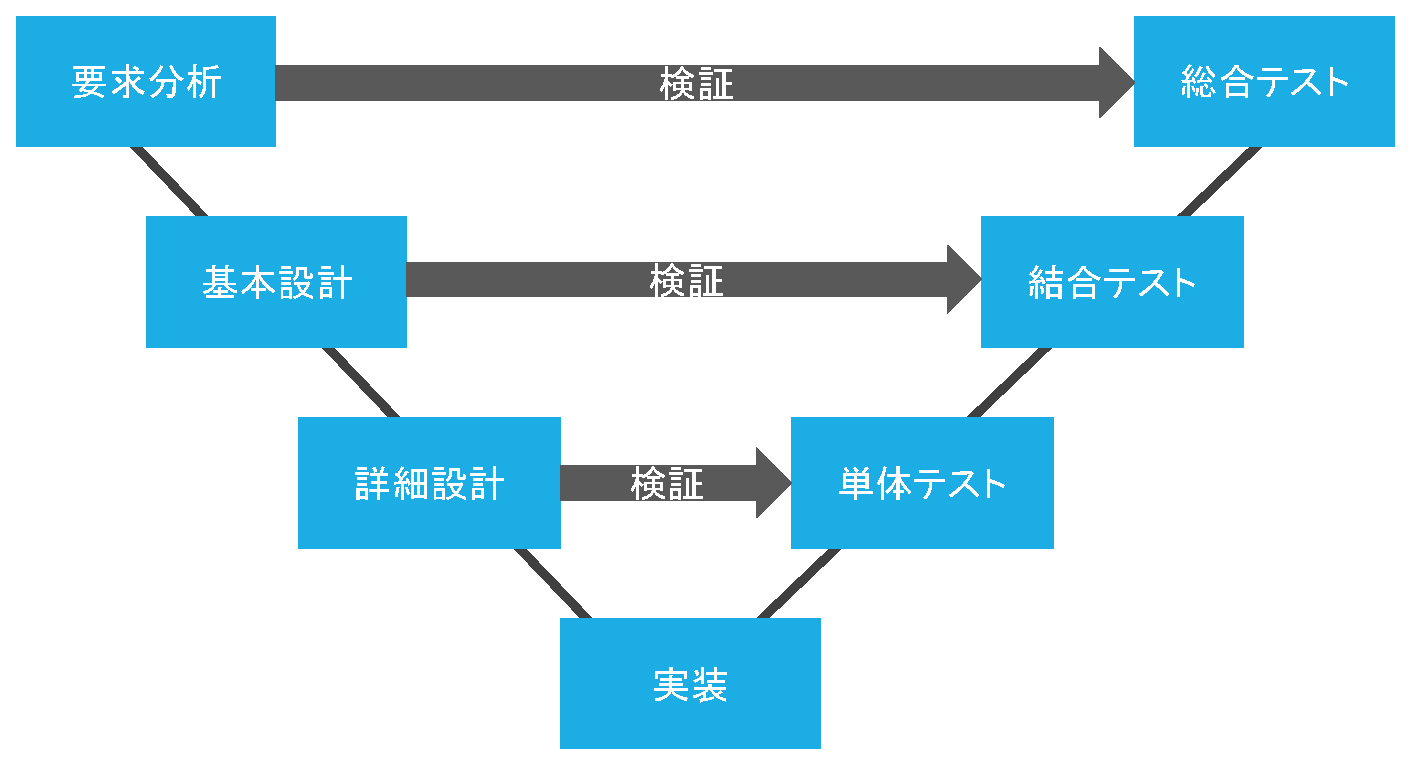
\includegraphics[width=10cm]{./pic/vjimodel.eps}
\caption{V字モデル}
\label{v_model}
\end{figure}

\subsection*{UML(Unifiled Modeling Language)}
UMLとは各開発工程で利用すべき図面を標準化した言語である。UMLの利点は、単純で分かりやすい点と、実用的な表現方法を持つ点である。UMLの構成要素としてユースケース図、クラス図、シーケンス図がある\cite{uml}。本研究ではシステムの設計を行う際に、曖昧な定義になるのを防ぐためにUMLを用いた。

\subsection*{ユースケース図}
システムがどのように機能すべきかという振る舞いとその外部環境を表す。ユースケース図を作成することで視覚的にわかりやすくなる。視覚的にわかりやすいことで、開発者だけでなく、クライアントにもシステムの概要が理解しやすくなる。本研究では、基本設計を行う際に使用した。


\subsection*{シーケンス図}
シーケンス図は、オブジェクト間のメッセージのやり取りを時系列順に沿って並べて表現したものである。四角の項目はオブジェクトと呼ぶ。矢印はメッセージと呼ばれ、意味はオブジェクト間のデータの伝達と動作が行われる。ユースケース図を基にしてシーケンス図やクラス図を制作を行う。本研究では、詳細設計を行う際に使用した。

\subsection*{クラス図}
クラス図はモデルの静的な構造を示す図である。クラスが持つ動作や、属性を記述する。より具体的な実装部分に近い記述を行う。本研究では、クラス図を参考にしながらシステムのモジュールを実装した。

\section{画像処理に用いた技術の用語解説}

\subsection*{Yolo(Real-Time Object Detection)}
Yoloはリアルタイムでのオブジェクト識別が可能ネットワークである。Webカメラを利用したリアルタイム検出も可能である。ほかのネットワークとの違いは、検出と識別を同時に行っているため高速性を保てる点である。本研究では、画像からバーコードの位置を特定し、バーコード部分のみを切り取るために使用した\cite{yolo}。


\subsection*{pyzbar}
pyzbarとは、python言語でバーコード画像を解析し、数字を識別するライブラリである\cite{pyzbar}。1次元バーコード以外にも、2次元バーコードであるQRコードの読み取りも行うことが可能。本研究では、バーコード画像からバーコード番号を識別するために使用した。